\chapter{\ifproject%
\ifcpe โครงสร้างและขั้นตอนการทำงาน\else Project Structure and Methodology\fi
\else%
\ifcpe โครงสร้างของโครงงาน\else Project Structure\fi
\fi
}


\makeatletter

% \renewcommand\section{\@startsection {section}{1}{\z@}%
%                                    {13.5ex \@plus -1ex \@minus -.2ex}%
%                                    {2.3ex \@plus.2ex}%
%                                    {\normalfont\large\bfseries}}

\makeatother
%\vspace{2ex}
% \titleformat{\section}{\normalfont\bfseries}{\thesection}{1em}{}
% \titlespacing*{\section}{0pt}{10ex}{0pt}
ในบทนี้จะกล่าวถึงผลสรุปจากการสํารวจความคิดเห็นของนักศึกษาเกี่ยวกับตารางสอบปลายภาค ข้อมูลที่จำเป็นต้องใช้สำหรับการพัฒนาโปรแกรม รวมถึงโครงสร้างข้อมูลรับเข้าและข้อมูลส่งออกของโปรแกรม
ซึ่งจากความต้องการพัฒนาระบบจัดตารางสอบปลายภาคเพื่อให้นักศึกษามีอิสระในการเลือกลงทะเบียนเรียนมากขึ้นดังที่กล่าวในตอนที่ \ref{sec:project_rationale} เราจึงต้องการทราบความคิดเห็นของนักศึกษาในมหาวิทยาลัยเชียงใหม่เกี่ยวกับตารางสอบปลายภาค 
ทำให้เราได้จัดทำแบบสอบถามขึ้นเพื่อสอบถามความคิดเห็นของนักศึกษามหาวิทยาลัยเชียงใหม่ ทั้งนักศึกษาปัจจุบันและนักศึกษาที่สำเร็จการศึกษาแล้ว ว่ามีความคิดเห็นอย่างไรกับตารางสอบปลายภาคในปัจจุบัน และหากเลือกได้อยากจะสอบในช่วงเวลาใดบ้าง ๆ ในตารางเวลาของสัปดาห์ที่จัดสอบ 
โดยจะพยายามนำข้อมูลที่ได้มาใช้ในการอ้างอิงเพื่อออกแบบอัลกอริทึมสำหรับประมวลผลหาวิธีการจัดตารางสอบที่เหมาะสมที่สุดที่เป็นไปได้สำหรับนักศึกษาทุกคน

\section{การสำรวจความคิดเห็นของนักศึกษาเกี่ยวกับตารางสอบปลายภาค}
\CIreply{เพิ่มรายละเอียดว่าผู้ตอบแบบสอบถามมาจากคณะใดบ้าง ชั้นปี ฯลฯ}
\TSNAreply{เพิ่มละครับ}
จากผลสำรวจของแบบสอบถามเกี่ยวกับตารางสอบปลายภาคของมหาวิทยาลัยชียงใหม่ โดยขอความร่วมมือนักศึกษาในมหาวิทยาลัย
ทั้งนักศึกษาที่กำลังศึกษาอยู่และทั้งที่สำเร็จการศึกษาไปแล้ว เพื่อให้ช่วยตอบแบบสอบถามความคิดเห็นเกี่ยวกับ ข้อดี ข้อเสีย ความพึงพอใจในตารางสอบของตนเอง
รวมถึงปัญหาเกี่ยวกับตารางสอบปลายภาคที่เคยพบหรือได้รับผลกระทบโดยตรง โดยจากผลการสำรวจกลุ่มสำรวจจำนวน 95 คน สามารถแบ่งผู้ตอบแบบสอบถามตามระดับการศึกษาได้ 5 ระดับดังกราฟที่ \ref{fig:academic_year} โดยมีจำนวนดังนี้
\begin{itemize}
  \item ชั้นปีที่ 1 จำนวน 14 คน
  \item ชั้นปีที่ 2 จำนวน 27 คน
  \item ชั้นปีที่ 3 จำนวน 11 คน
  \item ชั้นปีที่ 4 จำนวน 38 คน
  \item มากกว่าชั้นปีที่ 4 จำนวน 2 คน
  \item สำเร็จการศึกษาแล้ว จำนวน 3 คน
\end{itemize}
\begin{figure}
  \begin{center}
    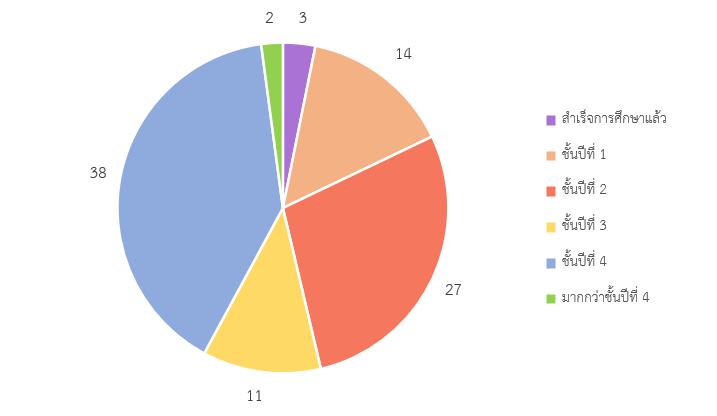
\includegraphics[width=\linewidth]{images/group_by_academic_year.png}
  \end{center}
  \caption[จำนวนผู้ตอบแบบสอบถามแบ่งตามชั้นปีที่ศึกษา]{จำนวนผู้ตอบแบบสอบถามแบ่งตามชั้นปีที่ศึกษา}
  \label{fig:academic_year}     
\end{figure}
และหากแบ่งผู้ตอบแบบสอบถามตามคณะที่ศึกษาจะสามารถแบ่งได้ดังกราฟที่ \ref{fig:faculty} 
โดยคณะอื่น ๆ ประกอบไปด้วยนักศึกษาจากคณะต่าง ๆ ดังนี้
\begin{itemize}
  \item คณะสังคมศาสตร์ จำนวน 2 คน
  \item คณะเกษตรศาสตร์ จำนวน 2 คน
  \item คณะเภสัชศาสตร์ จำนวน 1 คน
  \item คณะเทคนิคการแพทย์ จำนวน 2 คน
  \item คณะพยาบาลศาสตร์ จำนวน 1 คน
  \item คณะสัตวแพทยศาสตร์ จำนวน 2 คน
  \item คณะรัฐศาสตร์และรัฐประศาสนศาสตร์ จำนวน 1 คน
  \item วิทยาลัยศิลปะ สื่อ และเทคโนโลยี จำนวน 1 คน
\end{itemize}
\begin{figure}
  \begin{center}
    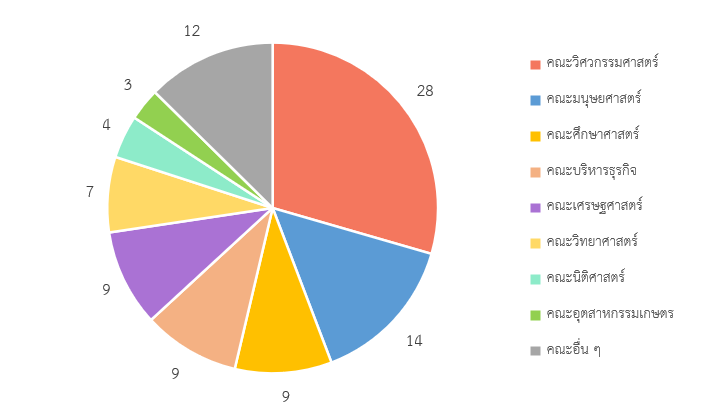
\includegraphics[width=\linewidth]{images/group_by_faculty.png}
  \end{center}
  \caption[จำนวนผู้ตอบแบบสอบถามแบ่งตามคณะที่ศึกษา]{จำนวนผู้ตอบแบบสอบถามแบ่งตามคณะที่ศึกษา}
  \label{fig:faculty}     
\end{figure}

โดยจากการสรุปผลการสำรวจพบว่าผู้ตอบแบบสอบถามส่วนใหญ่นั้นตรวจสอบตารางสอบของทุกวิชาที่ต้องการจะลงทะเบียน
ก่อนที่จะลงทะเบียนเรียนอย่างสม่ำเสมอ แต่ยังมีผู้ตอบแบบสอบถามบางส่วนนั้นที่ตรวจสอบตารางสอบเพียงบางวิชาก่อนจะลงทะเบียนเรียน และยังมีมีผู้ตอบแบบสอบถามส่วนน้อยที่ตอบว่าไม่เคยตรวจสอบตารางสอบของตนเองเลย ดังกราฟที่ \ref{fig:check_before_enrollment}
\begin{figure}
  \begin{center}
    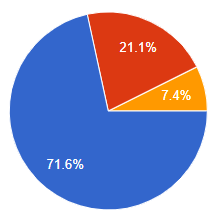
\includegraphics{images/checking_schedule_before_enrollment.png}\\[2ex]
    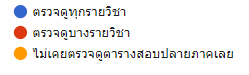
\includegraphics{images/legend_for_checking_schedule_before_enrollment.png}
  \end{center}
  \caption[จำนวนผู้ตอบแบบสอบถามที่ตรวจสอบตารางสอบปลายภาคก่อนการลงทะเบียน]{จำนวนผู้ตอบแบบสอบถามที่ตรวจสอบตารางสอบปลายภาคก่อนการลงทะเบียน}
  \label{fig:check_before_enrollment}     
\end{figure}
จากผลการสำรวจเรายังพบว่ากลุ่มสำรวจกว่า 80\% ไม่ทราบว่าสำนักทะเบียนมหาลัยเชียงใหม่ จัดตารางสอบปลายภาคอย่างไร ดังแสดงในกราฟที่ \ref{fig:registration_exam}
\begin{figure}
  \begin{center}
    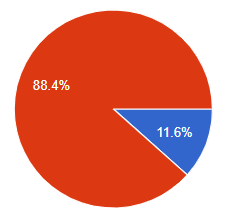
\includegraphics{images/registration_exam.png}\\[2ex]
    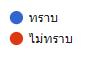
\includegraphics{images/legend_for_registration_exam.png}
  \end{center}
  \caption[จำนวนผู้ตอบแบบสอบถามที่ทราบวิธีการจัดตารางสอบปลายภาคของสำนักทะเบียน]{จำนวนผู้ตอบแบบสอบถามที่ทราบวิธีการจัดตารางสอบปลายภาคของสำนักทะเบียน}
  \label{fig:registration_exam}     
\end{figure}
จากผลการสำรวจเรายังสามารถสรุปผลได้ดังนี้
วันที่ผู้ทำแบบสอบถามต้องการจะสอบมากที่สุด 7 อันดับแรก โดยเรียงลำดับจากมากไปน้อย
\begin{enumerate}
  \item สัปดาห์ที่หนึ่ง วันจันทร์
  \item สัปดาห์ที่หนึ่ง วันพุธ
  \item สัปดาห์ที่หนึ่ง วันศุกร์ 
  \item สัปดาห์ที่หนึ่ง วันอาทิตย์
  \item สัปดาห์ที่สอง วันอังคาร
  \item สัปดาห์ที่สอง วันพฤหัสบดี
  \item สัปดาห์ที่สอง วันเสาร์
\end{enumerate}

จากข้อมูลเราสามารถบอกได้ว่าเวลาที่ผู้ทำแบบสอบถามส่วนใหญ่ต้องการที่จะสอบในแต่ละวันคือ
ช่วงเวลา 12.00-15.00น. ซึ่งผู้ทำแบบสอบถามส่วนมากต้องการจะสอบช่วงเวลานี้มากกว่า 15.30-18.00น. และ 08.00-11.00น. ตามลำดับ ดังกราฟ \ref{fig:time}
\begin{figure}
  \begin{center}
    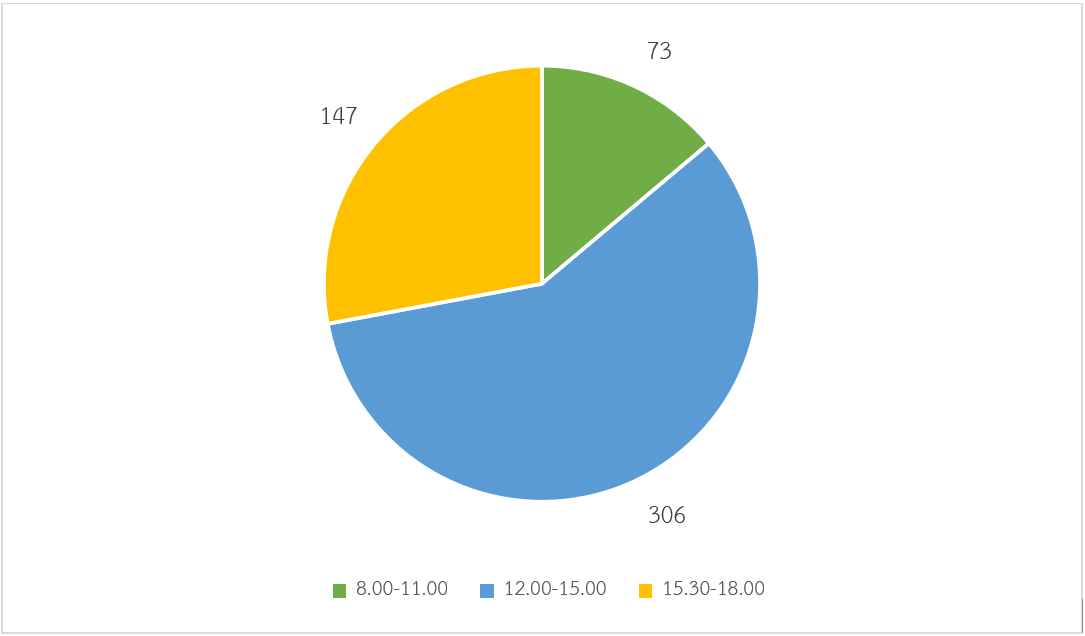
\includegraphics[width=\linewidth]{images/pie_chart_for_final_exam_time.png}
  \end{center}
  \caption[วามต้องการในการสอบของผู้ตอบแบบสอบถามในแต่ละเวลา]{ความต้องการในการสอบของผู้ตอบแบบสอบถามในแต่ละเวลา}
  \label{fig:time}
\end{figure}
และถ้าเราทำการรวมช่วงเวลาที่ผู้ตอบแบบสอบถามต้องการสอบกับวันที่ผู้ตอบแบบสอบถามต้องการสอบเข้าด้วยกันดังกราฟที่ \ref{fig:time_slot} จะสามารถสรุปวันที่ผู้ทำแบบสอบถามต้องการจะสอบมากที่สุด 7 อันดับแรก โดยสามารถเรียงลำดับจากมากไปน้อยได้ ดังนี้
\begin{figure}
  \begin{center}
    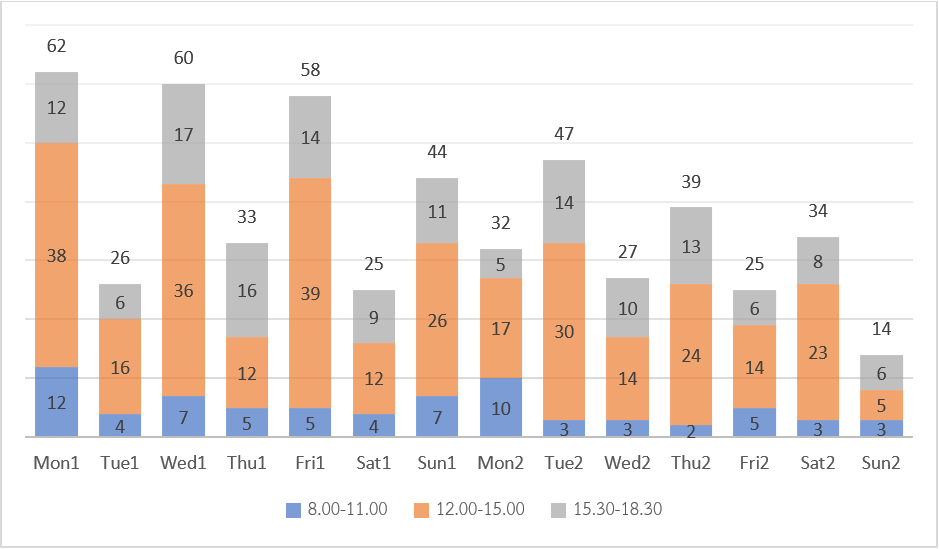
\includegraphics[width=\linewidth]{images/bar_chart_for_final_exam_slot.png}
  \end{center}
  \caption[ความต้องการในการสอบของผู้ตอบแบบสอบถามในแต่ละช่วงเวลาสอบ]{ความต้องการในการสอบของผู้ตอบแบบสอบถามในแต่ละช่วงเวลาสอบ}
  \label{fig:time_slot}     
\end{figure}
\begin{enumerate}
  \item สัปดาห์ที่หนึ่ง เวลา 12.00-15.00น. วันศุกร์ 
  \item สัปดาห์ที่หนึ่ง เวลา 12.00-15.00น. วันจันทร์
  \item สัปดาห์ที่หนึ่ง เวลา 12.00-15.00น. วันพุธ
  \item สัปดาห์ที่สอง เวลา 12.00-15.00น. วันอังคาร
  \item สัปดาห์ที่หนึ่ง เวลา 12.00-15.00น. วันอาทิตย์
  \item สัปดาห์ที่สอง เวลา 12.00-15.00น. วันพฤหัสบดี
  \item สัปดาห์ที่สอง เวลา 12.00-15.00น. วันเสาร์
\end{enumerate}

ซึ่งจากกราฟ \ref{fig:time_slot} ยังสามารถสรุปได้ว่าผู้ทำแบบสอบถามส่วนใหญ่ต้องการที่จะสอบหนึ่งวันเว้นหนึ่งวันเพื่อที่จะได้มีเวลาในการอ่านหนังสือเตรียมสอบสำหรับวิชาในวันถัดไปมากกว่าการสอบติดกัน 
เรายังสามารถบอกเพิ่มเติมได้อีกว่าผู้ทำแบบสอบถามส่วนใหญ่ต้องการสอบในช่วงสัปดาห์แรกของช่วงการสอบมากกว่าช่วงสัปดาห์ที่สองเพื่อที่จะได้มีเวลาพักผ่อนหรือกลับบ้าน หลังจากที่สอบเสร็จแล้ว
\newpage
\section{โครงสร้างและการทำงานของโปรแกรม}
\subsection{ข้อมูลที่ต้องใช้ในการจัดตารางสอบ}
ข้อมูลนำเข้าของโปรแกรมจะมีโครงสร้างไดเรกทอรี่และไฟล์ดังที่แสดง

\begin{forest}
  for tree={
    font=\ttfamily,
    grow'=0,
    child anchor=west,
    parent anchor=south,
    anchor=west,
    calign=first,
    inner xsep=7pt,
    edge path={
      \noexpand\path [draw, \forestoption{edge}]
      (!u.south west) +(7.5pt,0) |- (.child anchor) pic {folder} \forestoption{edge label};
    },
    % style for your file node 
    file/.style={edge path={\noexpand\path [draw, \forestoption{edge}]
      (!u.south west) +(7.5pt,0) |- (.child anchor) \forestoption{edge label};},
      inner xsep=2pt,font=\small\ttfamily
                 },
    before typesetting nodes={
      if n=1
        {insert before={[,phantom]}}
        {}
    },
    fit=band,
    before computing xy={l=15pt},
  } 
[root-folder
  [data
    [all-exam-courses
      [all-exam-courses.in,file]
    ]
    [capacity
      [faculty-capacity.in,file]
    ]
    [exam-courses-faculty
      [01.in,file]
      [02.in,file]
      [03.in,file]
      [...,file]
      [19.in,file]
      [20.in,file]
      [21.in,file]
    ]
    [regist
      [regist-academic\_year-semester.in,file]
    ]
    [sched
      [conflicts.in,file]
      [courses.in,file]
    ]
  ]
  [final\_exam\_graph\_coloring.py,file]
]
\end{forest}
\begin{figure}
  \begin{center}
    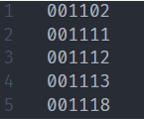
\includegraphics[]{images/all-exam1.png}
  \end{center}
  \caption[ตัวอย่างไฟล์รายวิชาที่มีสอบ]{ตัวอย่างไฟล์รายวิชาที่มีสอบ}
  \label{fig:all_courses}     
\end{figure}
\begin{figure}
  \begin{center}
    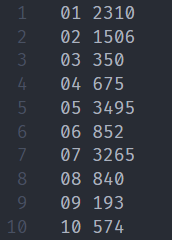
\includegraphics[]{images/capacity1.png}
  \end{center}
  \caption[ตัวอย่างไฟล์ความจุห้องสอบ]{ตัวอย่างไฟล์ความจุห้องสอบ}
  \label{fig:capacity}     
\end{figure}
\begin{figure}
  \begin{center}
    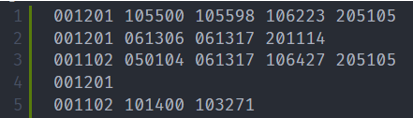
\includegraphics[]{images/regist1.png}
  \end{center}
  \caption[ตัวอย่างไฟล์ลงทะเบียนของนักศึกษา]{ตัวอย่างไฟล์ลงทะเบียนของนักศึกษา}
  \label{fig:regist}     
\end{figure}
\begin{figure}
  \begin{center}
    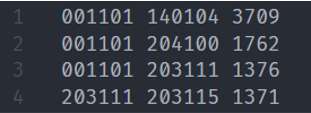
\includegraphics[]{images/conflicts1.png}
  \end{center}
  \caption[ตัวอย่างไฟล์คู่วิชาที่มีนักศึกษาลงทะเบียนพร้อมกัน]{ตัวอย่างไฟล์คู่วิชาที่มีนักศึกษาลงทะเบียนพร้อมกัน}
  \label{fig:conflicts}     
\end{figure}
\begin{figure}
  \begin{center}
    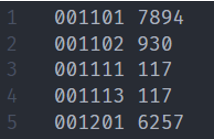
\includegraphics[]{images/courses1.png}
  \end{center}
  \caption[ตัวอย่างไฟล์วิชาที่มีนักศึกษาลงทะเบียน]{ตัวอย่างไฟล์วิชาที่มีนักศึกษาลงทะเบียน}
  \label{fig:courses}     
\end{figure}
\begin{itemize}
  \item ในโฟลเดอร์ all-exam-course ประกอบไปด้วยไฟล์ all-exam-course.in จำนวน 1 ไฟล์ ซึ่งเป็นไฟล์ text ในไฟล์แต่ละบรรทัดประกอบด้วยรหัสวิชาที่มีการจัดสอบ หนึ่งบรรทัดต่อหนึ่งรหัสวิชา ดังภาพที่ \ref{fig:all_courses}
  \item ในโฟลเดอร์ capacity ประกอบไปด้วยไฟล์ faculty-capacity.in จำนวน 1 ไฟล์ ซึ่งเป็นไฟล์ text ในไฟล์แต่ละบรรทัดประกอบไปด้วย รหัสคณะ และจำนวนความจุรวมของห้องสอบของคณะนั้น ๆ แต่ละส่วนคั่นด้วย เว้นวรรค (Space) ดังภาพที่ \ref{fig:capacity}
  \item ในโฟลเดอร์ exam-courses-faculty ประกอบไปด้วยไฟล์ 01.in ถึง 21.in ซึ่งเป็นไฟล์ text โดยตั้งชื่อไฟล์ตามรหัสคณะ ในแต่ละไฟล์ประกอบด้วย รหัสวิชาที่มีการจัดสอบ หนึ่งบรรทัดต่อหนึ่งรหัสวิชา ดังภาพที่ \ref{fig:all_courses} 
  \item ในโฟลเดอร์ regist ประกอบไปด้วยไฟล์ regist-ปีการศึกษา-เทอม.in ซึ่งเป็นไฟล์ text ในไฟล์ประกอบไปด้วยข้อมูลลงทะเบียนของนักศึกษาแต่ละคน แต่ละบรรทัดประกอบด้วย รหัสวิชาที่นักศึกษาหนึ่งคนลงทะเบียนในเทอมนั้น ๆ แต่ละวิชาคั่นด้วย เว้นวรรค (Space) ดังภาพที่ \ref{fig:regist}
  \item ในโฟลเดอร์ sched ประกอบไปด้วยไฟล์ conflicts.in ดังภาพที่ \ref{fig:conflicts} และ courses.in ดังภาพที่ \ref{fig:courses} ซึ่งเป็นไฟล์ text ในไฟล์ conflicts.in ประกอบด้วย รหัสวิชาสองวิชาที่มีนักศึกษาลงทะเบียนพร้อมกันในภาคการศึกษานั้น ๆ และ จำนวนนักศึกษาที่ลงทะเบียนคู่วิชานี้ แต่ละส่วนคั่นด้วย เว้นวรรค (Space) ในไฟล์ courses.in ประกอบด้วยรหัสวิชา และจำนวนนักศึกษาที่ลงทะเบียนในวิชานั้น ๆ แต่ละส่วนคั่นด้วย เว้นวรรค (Space)
\end{itemize}

\subsection{ผลลัพธ์จากการจัดตารางสอบ}
ข้อมูลผลลัพธ์ของโปรแกรมจะเป็นไฟล์ csv ที่ระบุรายวิชาคู่กับ slot ที่สอบของรายวิชานั้น ๆ โดยจะมีข้อมูลใช้สำหรับ mapping หมายเลข slot เป็นวันและเวลาสอบ

\subsection{แผนผังการทำงานของโปรแกรม (Flowchart)}
การทำงานของโปรแกรมจัดตารางสอบมีการแบ่งอัลกอริทึมออกเป็น 4 รูปแบบ
ที่ได้ทำการทดลองเพื่อหาตารางสอบแบบที่ดีที่สุดโดยเมื่อจะรันโปรแกรมจะต้องเลือกอัลกอริทึม 1 รูปแบบจากทั้งหมด 4 รูปแบบ ดังขั้นตอนที่ 1 
โดยการทำงานของโปรแกรมจะมีลำดับการทำงานตามภาพที่ \ref{fig:flowchart}
สำหรับวิธีการของอัลกอริทึมแต่ละรูปแบบจะมีการกล่าวถึงในส่วนถัดไป

\subsection{รูปแบบของอัลกอลิทึม}
\begin{enumerate}
  \item อัลกอริทึมแบบที่ 1 BFS-DEG ใช้วิธี Graph coloring โดยเรียงลำดับวิชา (node) ที่จะจัดช่วงเวลาสอบ (slot) ให้ จากการ bfs ที่ node ที่มีดีกรีใน node นั้นมากที่สุด
  ก่อนและไล่จัด slot ไปตามเพื่อนบ้าน (neighbor node) ที่มีดีกรีจากมากไปน้อย หากมี node ที่ดีกรีเท่ากัน จะเรียงตามจำนวนนักศึกษาของ node จากมากไปน้อย และหากจำนวนนักศึกษาเท่ากันอีกจะเรียงตามผลรวมจำนวนของ conflict ของ node นั้น ๆ 
  และสุดท้ายหากผลรวมจำนวนของ conflict เท่ากันจะเรียงตามรหัสวิชา เมื่อจัด slot ไปจนครบทุก neighbor node แล้วจะเริ่ม กระบวนการนี้ซ้ำที่ neighbor node ไปจนกว่าจะจัด slot ได้ครบทุก node
  \item อัลกอริทึมแบบที่ 2 DEG ใช้วิธี Graph coloring โดยเรียงลำดับวิชา (node) ที่จะจัดช่วงเวลาสอบ (slot) ให้ ตามดีกรีของ node นั้นจากมากไปน้อยก่อน
  หากมี node ที่ดีกรีเท่ากัน จะเรียงตามจำนวนนักศึกษาของ node จากมากไปน้อย และหากจำนวนนักศึกษาเท่ากันอีกจะเรียงตามผลรวมจำนวนของ conflict ของ node นั้น ๆ 
  และสุดท้ายหากผลรวมจำนวนของ conflict เท่ากันจะเรียงตามรหัสวิชา
  \item อัลกอริทึมแบบที่ 3 BFS-STD ใช้วิธี Graph coloring โดยเรียงลำดับวิชา (node) ที่จะจัดช่วงเวลาสอบ (slot) ให้ จากการ bfs ที่ node ที่มีจำนวนนักศึกษาใน node นั้นมากที่สุด
  ก่อนและไล่จัด slot ไปตามเพื่อนบ้าน (neighbor node) ที่มีจำนวนนักศึกษาจากมากไปน้อย หากมี node ที่จำนวนนักศึกษาเท่ากัน จะเรียงตามจำนวนดีกรีของ node จากมากไปน้อย และหากดีกรีเท่ากันอีกจะเรียงตามผลรวมจำนวนของ conflict ของ node นั้น ๆ 
  และสุดท้ายหากผลรวมจำนวนของ conflict เท่ากันจะเรียงตามรหัสวิชา เมื่อจัด slot ไปจนครบทุก neighbor node แล้วจะเริ่ม กระบวนการนี้ซ้ำที่ neighbor node ไปจนกว่าจะจัด slot ได้ครบทุก node
  \item อัลกอริทึมแบบที่ 4 STD ใช้วิธี Graph coloring โดยเรียงลำดับวิชา (node) ที่จะจัดช่วงเวลาสอบ (slot) ให้ ตามจำนวนนักศึกษาใน node นั้นจากมากไปน้อยก่อน
  หากมี node ที่จำนวนนักศึกษาเท่ากัน จะเรียงตามจำนวนดีกรีของ node จากมากไปน้อย และหากดีกรีเท่ากันอีกจะเรียงตามผลรวมจำนวนของ conflict ของ node นั้น ๆ 
  และสุดท้ายหากผลรวมจำนวนของ conflict เท่ากันจะเรียงตามรหัสวิชา
  
  
\end{enumerate}

\begin{figure}
  \begin{center}
    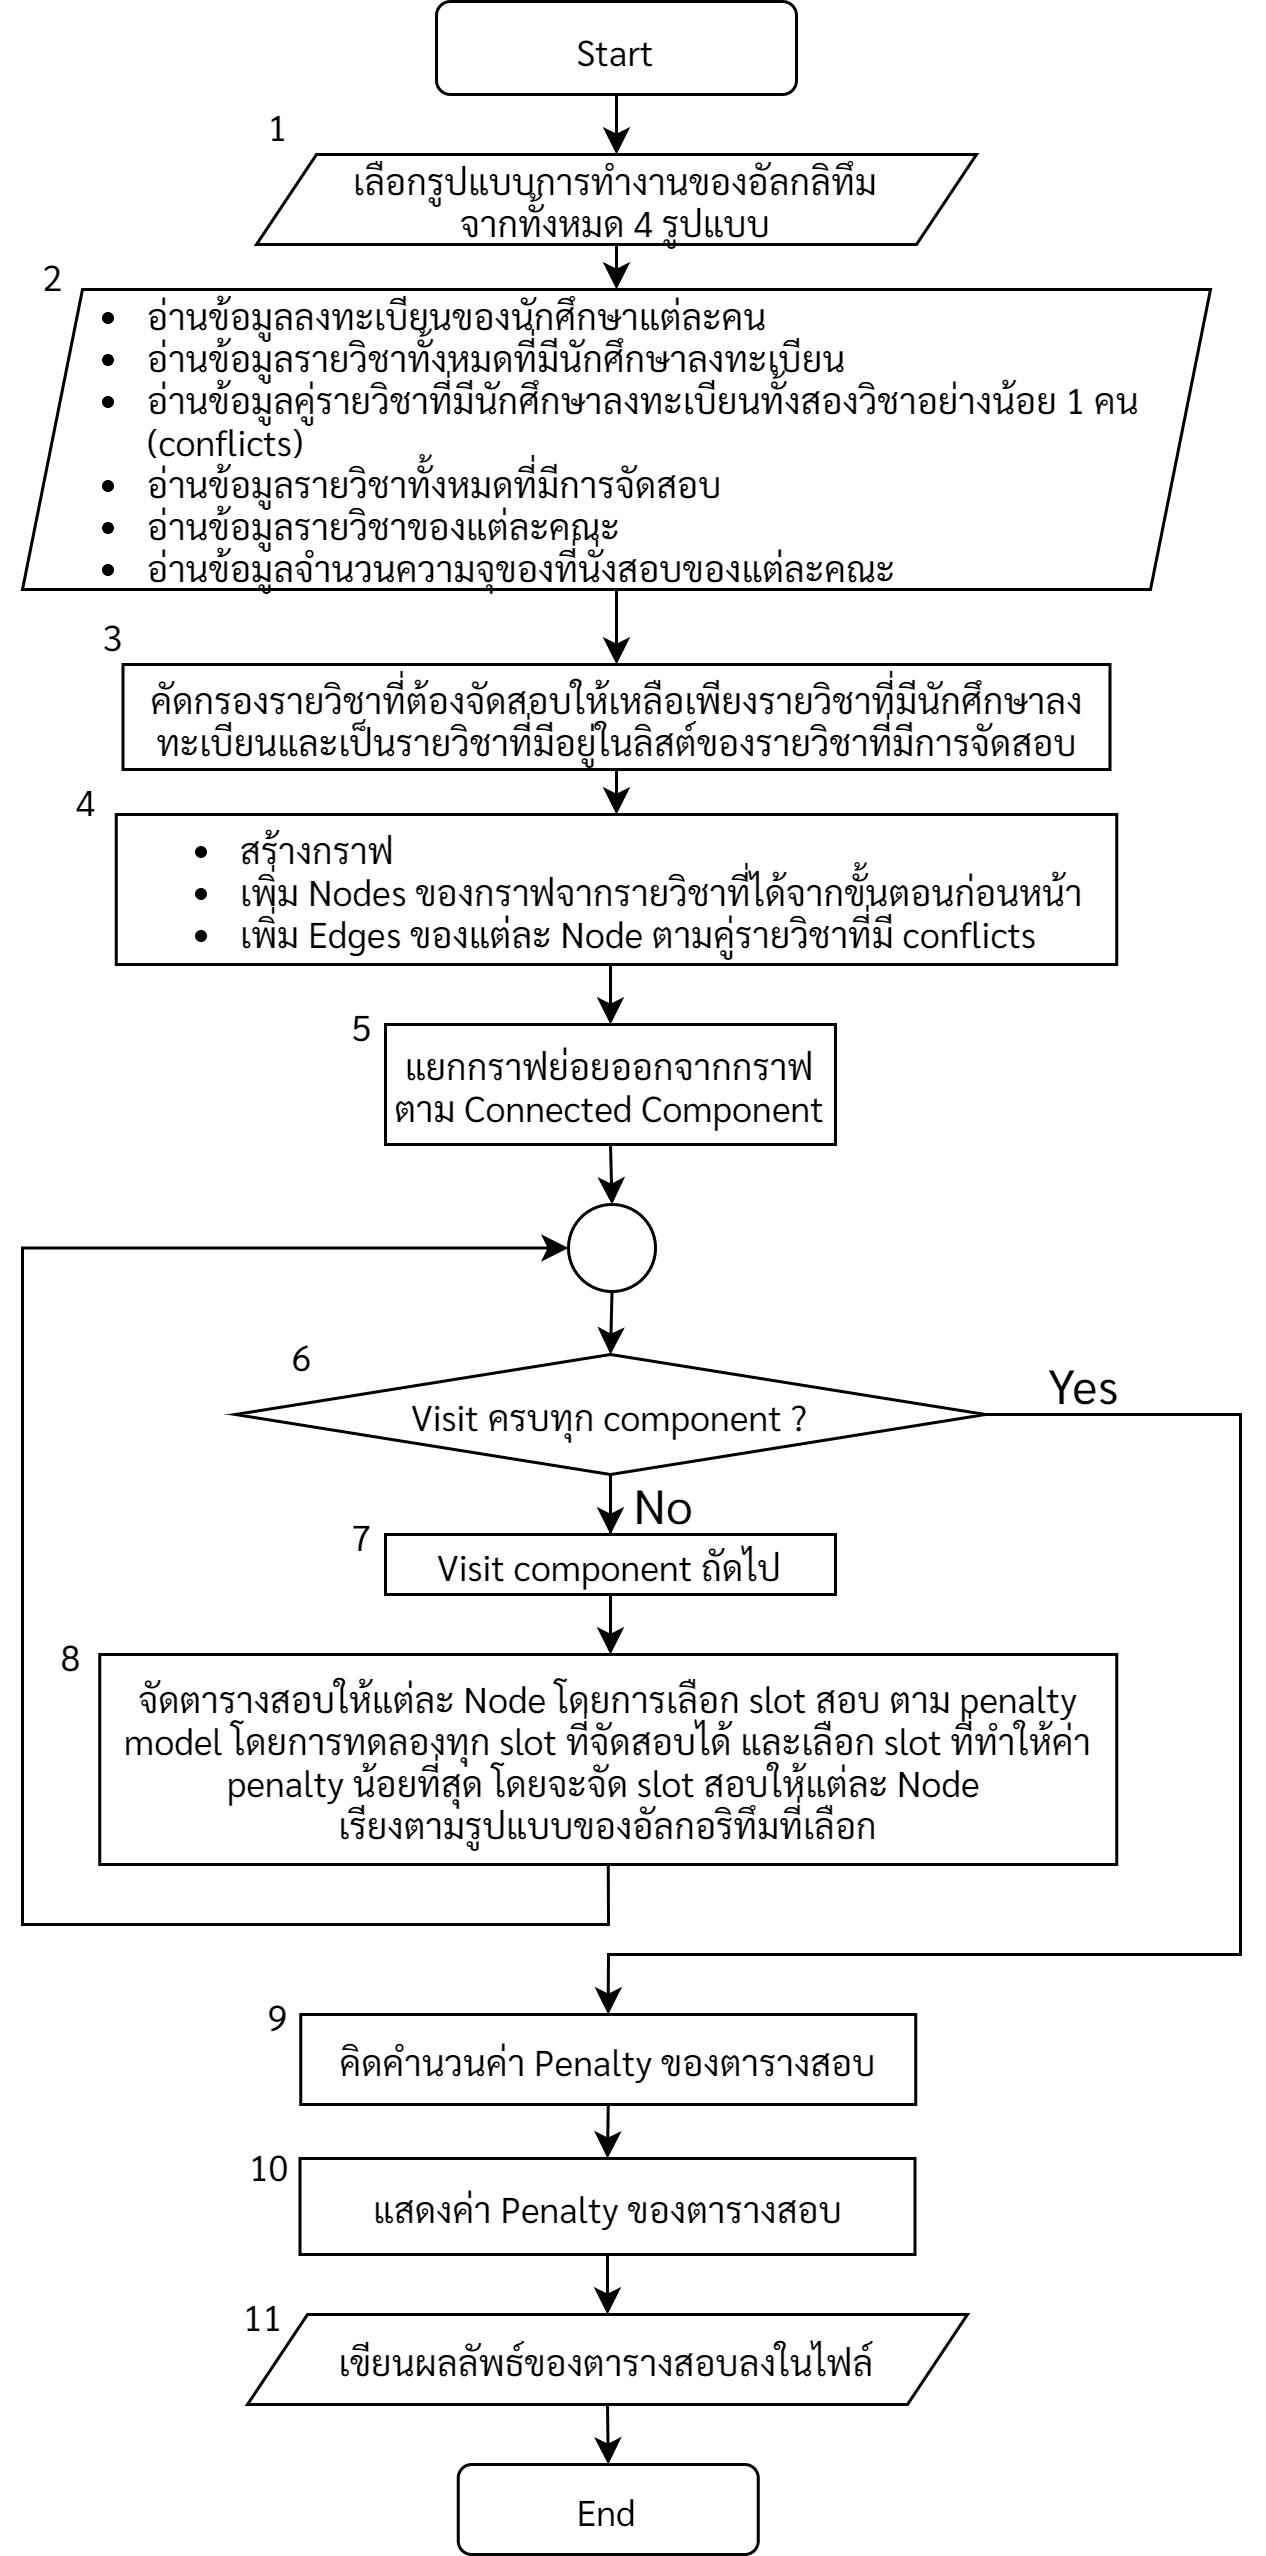
\includegraphics[]{images/exam_sched_flowchart.png}
  \end{center}
  \caption[แผนผังการทำงานของโปรแกรม]{แผนผังการทำงานของโปรแกรม}
  \label{fig:flowchart}     
\end{figure}
